\begin{tikzpicture}
	\pgfplotsset{/tikz/font={\small}}
	\begin{axis}[
		grid=both,
		width=1.0\textwidth,
		height=0.3\textheight,
		x tick label style={
		/pgf/number format/1000 sep=},
		ytick={0,-2,...,-12},
		y tick label style={
			/pgf/number format/.cd,
			fixed,
			fixed zerofill,
			precision=1,
		},
		y dir=reverse,
		ymax=1, ymin=-12,
		ylabel={Y BD-rate (\%)},
		% enlargelimits=0.15,
		enlarge y limits=false,
		enlarge x limits=0.04,
		legend style={at={(0.5,-0.45)},
		anchor=north,legend columns=-1},
		ybar,
		bar width=1pt,
		xtick=data,
		xtick align=inside,
		% nodes near coords,
		% xlabel={Sequences},
		% xlabel near ticks,
		symbolic x coords={
			NebutaFestival,
			PeopleOnStreet,
			SteamLocTrain,
			Traffic,
			BasketballDrive,
			BQTerrace,
			Cactus,
			Kimono1,
			ParkScene,
			BasketballDrill,
			BQMall,
			PartyScene,
			RaceHorses\_480p,
			BasketballPass,
			BlowingBubbles,
			BQSquare,
			RaceHorses\_240p,
			FourPeople,
			Johnny,
			KristenAndSara,
			BasketDrillText,
			ChinaSpeed,
			SlideEditing,
			SlideShow,
			Overall,
		},
		x tick label style={rotate=-60,anchor=west},
		]

		\addlegendentry{Sep KLT AI}
		\addplot coordinates {
		(NebutaFestival,   -0.55)
		(PeopleOnStreet,   -1.17)
		(SteamLocTrain,    -0.50)
		(Traffic,          -1.33)
		(BasketballDrive,   0.12)
		(BQTerrace,         0.27)
		(Cactus,           -0.92)
		(Kimono1,          -0.38)
		(ParkScene,        -1.19)
		(BasketballDrill,  -1.20)
		(BQMall,            0.03)
		(PartyScene,       -0.04)
		(RaceHorses\_480p, -0.84)
		(BasketballPass,   -0.11)
		(BlowingBubbles,   -0.05)
		(BQSquare,          0.09)
		(RaceHorses\_240p, -1.00)
		(FourPeople,       -1.19)
		(Johnny,           -0.33)
		(KristenAndSara,   -0.18)
		(BasketDrillText,  -0.84)
		(ChinaSpeed,        0.44)
		(SlideEditing,      0.68)
		(SlideShow,         0.73)
		(Overall,          -0.39)
		};

		\addlegendentry{Sep RDOT AI}
		\addplot coordinates {
		(NebutaFestival,   -0.37)
		(PeopleOnStreet,   -1.31)
		(SteamLocTrain,    -0.41)
		(Traffic,          -1.49)
		(BasketballDrive,  -0.59)
		(BQTerrace,        -0.85)
		(Cactus,           -1.47)
		(Kimono1,          -0.47)
		(ParkScene,        -1.28)
		(BasketballDrill,  -1.77)
		(BQMall,           -1.14)
		(PartyScene,       -1.15)
		(RaceHorses\_480p, -1.26)
		(BasketballPass,   -0.94)
		(BlowingBubbles,   -0.97)
		(BQSquare,         -1.00)
		(RaceHorses\_240p, -1.34)
		(FourPeople,       -1.51)
		(Johnny,           -0.75)
		(KristenAndSara,   -0.59)
		(BasketDrillText,  -1.80)
		(ChinaSpeed,       -0.81)
		(SlideEditing,     -0.57)
		(SlideShow,        -0.55)
		(Overall,          -1.02)
		};

		\addlegendentry{N-sep KLT AI}
		\addplot coordinates {
		(NebutaFestival,  -0.72)
		(PeopleOnStreet,  -2.53)
		(SteamLocTrain,   -0.60)
		(Traffic,         -2.66)
		(BasketballDrive, -1.12)
		(BQTerrace,       -2.19)
		(Cactus,          -2.28)
		(Kimono1,         -0.95)
		(ParkScene,       -1.69)
		(BasketballDrill, -7.92)
		(BQMall,          -0.83)
		(PartyScene,      -1.00)
		(RaceHorses\_480p,-2.60)
		(BasketballPass,  -1.47)
		(BlowingBubbles,  -1.80)
		(BQSquare,        -0.91)
		(RaceHorses\_240p,-3.36)
		(FourPeople,      -2.41)
		(Johnny,          -1.52)
		(KristenAndSara,  -1.56)
		(BasketDrillText, -6.14)
		(ChinaSpeed,      -0.02)
		(SlideEditing,     0.98)
		(SlideShow,        0.37)
		(Overall,         -1.87)
		};

		\addlegendentry{N-sep RDOT AI}
		\addplot coordinates {
		(NebutaFestival,   -0.44)
		(PeopleOnStreet,   -2.50)
		(SteamLocTrain,    -0.55)
		(Traffic,          -2.90)
		(BasketballDrive,  -2.82)
		(BQTerrace,        -4.62)
		(Cactus,           -3.41)
		(Kimono1,          -1.11)
		(ParkScene,        -1.92)
		(BasketballDrill, -11.88)
		(BQMall,           -2.58)
		(PartyScene,       -2.56)
		(RaceHorses\_480p, -3.57)
		(BasketballPass,   -3.12)
		(BlowingBubbles,   -3.49)
		(BQSquare,         -2.69)
		(RaceHorses\_240p, -4.34)
		(FourPeople,       -3.20)
		(Johnny,           -2.82)
		(KristenAndSara,   -2.99)
		(BasketDrillText,  -9.96)
		(ChinaSpeed,       -1.81)
		(SlideEditing,     -0.46)
		(SlideShow,        -1.81)
		(Overall,          -3.23)
		};

	\end{axis}
\end{tikzpicture}
